 \section{Verwendeter RC-Fernsteuerung}
 Die Verwendete RC-Fernsteuerung ist die \textit{T8L Radio Controller (M2)}
 \cite{t8l_controller} von Radiomaster. Sie wurde gewählt, da sie im Vergleich
 mit Fernsteuerungen mit den gleichen Features, am günstigsten ist. Sie
 supported das ExpressLRS Protokoll auf 2.4GHz. Als Empfänger wurde ein
 \textit{XR1 Nano Multi-Frequency ExpressLRS Receiver} \cite{XR1_reciver} von
 Radiomaster genutzt. Diese unterstützt auch das ExpressLRS Protokoll auf
 2.4GHz. Die empfangen Daten werden über das das CRSF Protokoll der
 Steuerplatine übertragen.

\noindent
\begin{minipage}[c]{0.5\textwidth}
    \centering
    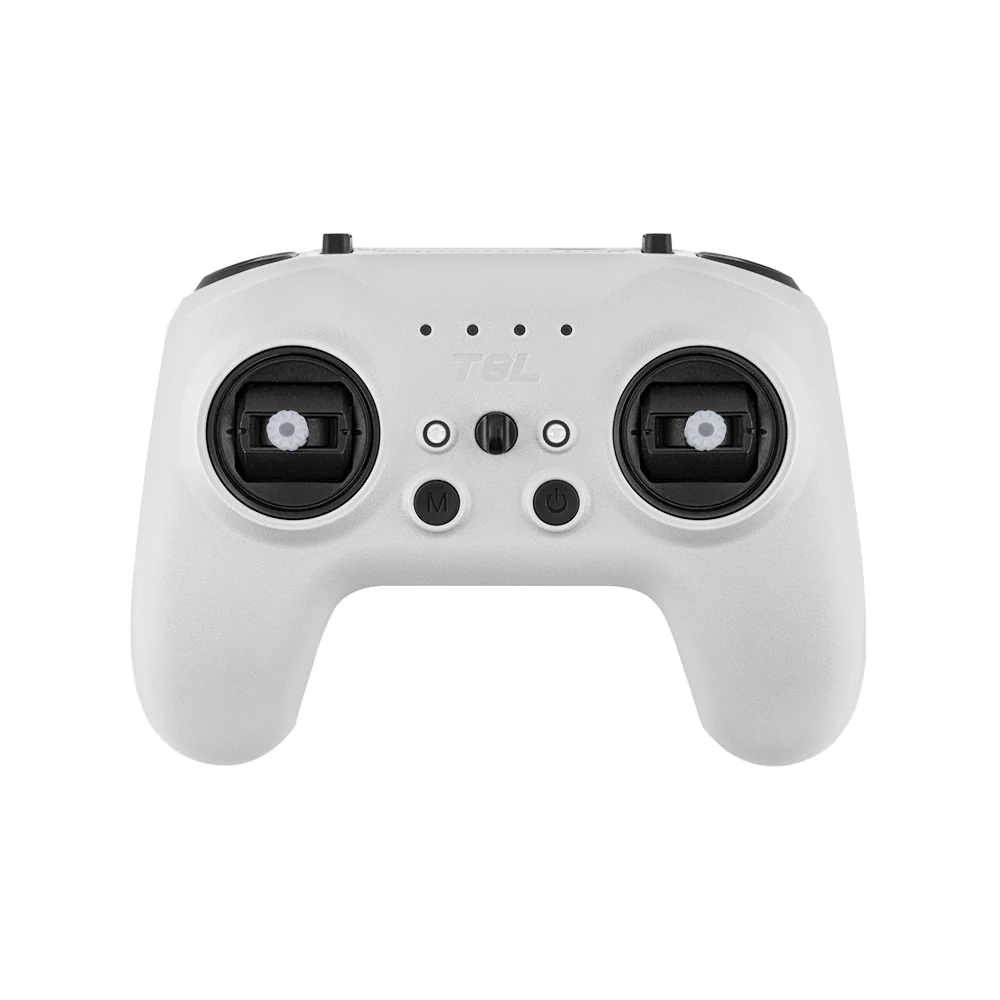
\includegraphics[width=\linewidth]{Bilder-Grafiken/Matthias/Fernsteuerung/T8L-RC-Controller.png}
    \captionof{figure}{Radiomaster T8L (M2) \cite{t8l_controller}}
\end{minipage}
\hfill
\begin{minipage}[c]{0.4\textwidth}
    \centering
    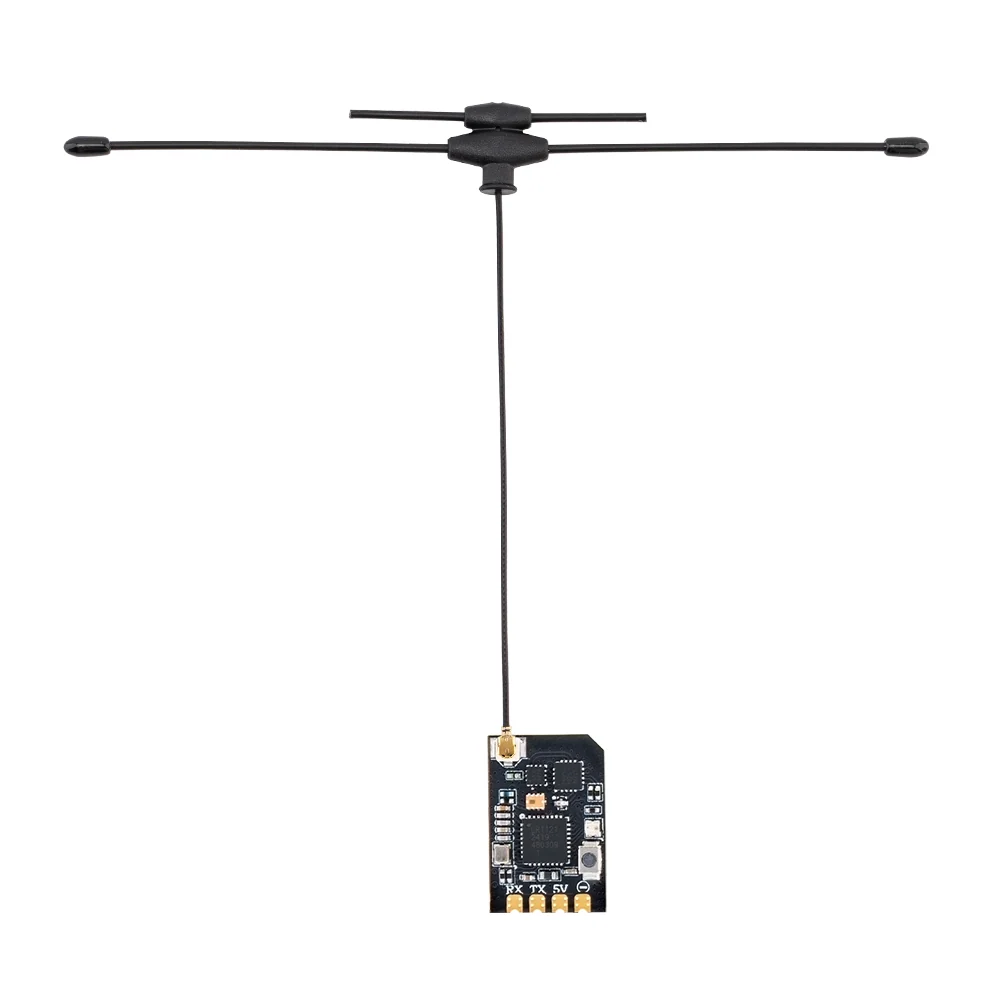
\includegraphics[width=\linewidth]{Bilder-Grafiken/Matthias/Fernsteuerung/XR1_Reciver_Bild.png}
    \captionof{figure}{Radiomaster XR1 Nano Multi-Frequency ExpressLRS Receiver
    \cite{XR1_reciver}}
\end{minipage}
\newpage
  

